\documentclass[12pt]{article}

\usepackage{fullpage}
\usepackage[normalem]{ulem}
\usepackage{mdframed}
\usepackage{amsmath}
\usepackage{float}
\usepackage{listings}
\usepackage{changepage}
\usepackage[final]{pdfpages}
\usepackage{hyperref}
\hypersetup{
    colorlinks,
    citecolor=black,
    filecolor=black,
    linkcolor=black,
    urlcolor=black
}
\usepackage[format=plain,
            font=it]{caption}
            
\usepackage{graphicx}
\graphicspath{ {.} }

\setlength{\parindent}{0pt}
\newcommand{\R}{\ensuremath{\mathit{R_{1}}}}
\newcommand{\tab}{\hspace{6mm}}
\renewcommand\labelitemi{$\boldsymbol{\cdot}$}

% Creating macros for figures and AST components.
\newcommand{\itm}[1]{\ensuremath{\mathit{#1}}}
\newcommand{\key}[1]{\texttt{#1}}
\newcommand{\lp}[0]{\key{(}}
\newcommand{\rp}[0]{\key{)}}
\newcommand{\lb}[0]{\key{[}}
\newcommand{\rb}[0]{\key{]}}
\newcommand{\lamb}[0]{\key{$\lambda$}}

\makeatletter
\newcommand{\Func}[1]{\lp\key{#1}\checknextarg}
\newcommand{\checknextarg}{\@ifnextchar\bgroup{\gobblenextarg}{\rp}}
\newcommand{\gobblenextarg}[1]{~#1\@ifnextchar\bgroup{\gobblenextarg}{\rp}}
\makeatother

\newcommand{\Atm}[0]{\itm{atom}}
\newcommand{\Exp}[0]{\itm{exp}}
\newcommand{\Def}[0]{\itm{def}}
\newcommand{\Op}[0]{\itm{op}}
\newcommand{\var}[0]{\itm{var}}
\newcommand{\Sub}[2]{\Func{-}{#1}{#2}}
\newcommand{\Add}[2]{\Func{+}{#1}{#2}}
\newcommand{\Mul}[2]{\Func{$\boldsymbol{\cdot}$}{#1}{#2}}

% Redesigning Sections
\newcommand{\usection}[1]{\section{#1}\hrule\hfill}


\title{Code Similarity Detection Tool\\
Design Documentation}
\author{Kevin Cao}

\begin{document}
\maketitle

\tableofcontents

\newpage

\usection{Introduction}

With the rising popularity of cryptocurrencies, it has become crucial that crypto-transactions are not only trustworthy, but also efficient and reliable. While Bitcoin continues to control a majority of the crypto-market, alternatives like Ethereum have also been growing in popularity.

\hfill

For some of these alternatives, transactions are controlled and automated using ``smart contracts". These smart contracts are computer programs that explicitly detail the rules and regulations to an agreement between two or more parties. Once the terms of the agreement have been met, the contract will self-execute and complete the transaction as agreed upon.

\subsection{Purpose}
For many transactions, the corresponding smart contracts are derived from pre-existing popular and mature contracts. By detecting the parent contracts that newer contracts are derived from, the verification process of the contracts can be expedited.

\hfill

As such, a Code Similarity Detection Tool would serve the purpose of assisting in the process of determining the original source of a new contract.

\subsection{Scope}

This Software Design Document details a basic system that serves as a proof of concept for a Code Similarity Detection Tool. For the sake of simplicity, the tool will compare the similarity between code written in a simplified subset of the lisp-based programming language Racket. The system first translates the source code into an Abstract Syntax Tree (AST), and then converts the AST into a variation of De Bruijn notation before running the similarity algorithm. Lisp-based languages are best suited for this type of translation, but other languages can also be similarly converted, although the process is a bit more involved.

\hfill

Furthermore, it should be clarified that the Code Similarity Detection Tool detailed in this document evaluates syntactical similarity, \emph{not semantical similarity}. The reasoning behind this is detailed later.

\newpage 

\usection{Conversion of Source Code}

\subsection{Programming Language Scope}

As mentioned in the previous section, the tool will act on a simplified subset of the Racket programming language, which will be referred to as \R{}. As such, it is best that this subset is defined explicitly.

\hfill

The most basic component in \R{} is an \Atm{}. Atoms include the basic primitive data values such as integers, booleans, and strings. It also includes variables and empty lists. Furthermore, as functions are first-class citizens in \R{}, built-in functions can also be considered as atoms.

\hfill

However, most programs in \R{} will not simply be made up of atoms \textemdash \R{} is largely comprised of \Exp{}s, or expressions. An expression can be a simple atom, an if-statement, a let-statement, a function application, or a lambda function. Figure \ref{concrete-syntax} shows some examples of expressions.

\hfill

Of course, in a functional programming language like \R{}, it is imperative that function definitions are explicated. Functional definitions are in a class of their own, \Def{}s. Definitions detail function construction by first taking a variable name to describe the function, and then variable parameters, which are used in the expression body of the definition. Expressions can use the function name from the definition in functional applications, which are categorized under expressions.

\hfill

Finally, an \R{} program can be described as a list of function definitions followed by a list of expression statements.

\begin{figure}[H]
  \begin{mdframed}
    \[
    \begin{array}{lcl}
      \Atm &::=& \itm{int} \mid \itm{bool} \mid \itm{str} \mid \itm{empty} \mid \var \mid \key{+} \mid \key{-} \mid \key{$\boldsymbol{\cdot}$} \mid \key{cons} \mid \key{eq?} \mid \key{and} \mid \key{or} \mid \key{not} \mid ... \\
      \Exp &::=& \Atm \mid \Func{if}{\Exp}{\Exp}{\Exp} \mid \lp\key{let}~\lp\lb\var~\Exp\rb\rp~\Exp\rp \\
           &\mid& \Add{\Exp}{\Exp} \mid \Sub{\Exp}{\Exp} \mid \Mul{\Exp}{\Exp} \mid \Func{-}{\Exp} \\
           &\mid& \Func{cons}{\Exp}{\Exp} \mid \Func{eq?}{\Exp}{\Exp} \mid \Func{and}{\Exp}{\Exp} \mid \Func{or}{\Exp}{\Exp} \mid \Func{not}{\Exp} \\ 
           &\mid& \Func{\lamb}{\lp\var}{...\rp}{\Exp} \mid ... \\
      \Def &::=& \lp\key{define}~\lp\var~\var~...\rp~\Exp\rp \\
      \R &::=& \Def~...~\Exp~...
    \end{array}
  \]
  \end{mdframed}
  \caption{The concrete syntax of \R. ``..." signifies a list of the previous token.}
  \label{concrete-syntax}
\end{figure}

Compared to Racket, \R{} is a fairly bare-bones language\textemdash however, \R{} will be sufficient in demonstrating the core mechanic of the system.

\subsection{Abstract Syntax Trees}
Before we can begin the similarity algorithm, we first need to convert the source code into an Abstract Syntax Tree, which abstracts away the source code into the node objects of the tree. In short, we convert the concrete syntax detailed in Figure \ref{concrete-syntax} into the abstract syntax detailed in Figure \ref{abstract-syntax}.

\begin{figure}[H]
  \begin{mdframed}
    \[
    \begin{array}{lcl}
      \Op &::=& \key{+} \mid \key{-} \mid \key{$\boldsymbol{\cdot}$} \mid \key{cons} \mid \key{eq?} \mid \key{and} \mid \key{or} \mid \key{not} \mid ... \\
      \Atm &::=& \Func{Int}{\itm{int}} \mid \Func{Bool}{\itm{bool}} \mid \Func{Str}{\itm{str}} \mid \Func{Empty} \mid \Func{Var}{\var} \mid \Func{Op}{\Op} \\
      \Exp &::=& \Atm \mid \Func{If}{\Exp}{\Exp}{\Exp} \mid \Func{Let}{\Func{Var}{\var}}{\Exp}{\Exp} \mid \Func{Apply}{\Exp}{\Exp}{...} \\
           &\mid& \Func{Lambda}{\lp\Func{Var}{\var}{}~...\rp}{\Exp} \mid ... \\
      \Def &::=& \Func{Def}{\Func{Var}{\var}}{\lp\Func{Var}{\var}{}~...\rp}{\Exp} \\
      \R &::=& \Func{Program}{\lp\Def{}~...\rp}{\lp\Exp{}...\rp}
    \end{array}
  \]
  \end{mdframed}
  \caption{The abstract syntax of \R.}
  \label{abstract-syntax}
\end{figure}

In Figure \ref{abstract-syntax}, the components of \R{} are converted into objects. You may notice a new classification, \Op{}. This simply acts as an abstraction for built-in functions in the \R{} language so that we can create the \Func{Op}{\Op}\space object in \Atm.

\hfill

The rest of Figure \ref{abstract-syntax} is fairly self-explanatory, so we will not go into further detail here.

\subsection{De Bruijn Notation}

While certain structures of code, such as if-statements or function definitions, must follow a set syntax, variable names are up to the discretion of the developer. In order to properly perform the code similarity algorithm, we must ignore the variable names and standardize the syntax.

\hfill

One method of doing so is to use De Bruijn indices\textemdash variables are instead replaced with numbers that indicate how many variable bindings exist between the variable occurrence and its corresponding binding. To avoid confusion with actual integers, we will rename variables as \texttt{v\#}.

\begin{figure}[H]
  \begin{mdframed}
    \begin{lstlisting}[escapechar=\%]
; Original Syntax
(%\lamb% (x)
  (%\lamb% (y)
    (%\lamb% (z)
      (+ x (+ y z)))))

; De Bruijnized Syntax
(%\lamb%
  (%\lamb% 
    (%\lamb% 
      (+ v2 (+ v1 v0)))))
    \end{lstlisting}
  \end{mdframed}
  \caption{Demonstrating conversion to De Bruijn indices.}
  \label{debruijn}
\end{figure}

However, this solution is not perfect\textemdash multi-variable functions would require currying in order to be properly De Bruijnized. Unfortunately, currying functions would make it difficult to perform similarity checks on function applications. In a later section, we will discuss the methodology for comparing two separate functional applications, but in short, we will need to collect all function arguments to properly compare. If functions are curried, then collecting the function arguments requires traversing down the AST and determining which expressions belong to the function application\textemdash a messier process than would be preferred (shown in Figure \ref{curried-ast}).

\hfill

\begin{figure}[H]
  \begin{mdframed}
    \begin{lstlisting}[escapechar=\%]
; Original Syntax
(define (func x y z)
  (+ x (+ y z)))

; Curried Syntax
(define (func x)
  (%\lamb% (y)
    (%\lamb% (z)
      (+ x (+ y z)))))

; Curried Function Application 1
(((func (+ 4 1)) (+ 2 3)) 6)

; Curried Function Application 2
(((func 6) (+ 4 1)) (+ 2 3))

; AST 1
(Apply
  (Apply
    (Apply
      (Var func) (Apply (Op +) (Int 4) (Int 1)))
    (Apply (Op +) (Int 2) (Int 3)))
  (Int 6))

; AST 2
(Apply
  (Apply
    (Apply
      (Var func) (Int 6))
    (Apply (Op +) (Int 4) (Int 1)))
  (Apply (Op +) (Int 2) (Int 3)))
    \end{lstlisting}
  \end{mdframed}
  \caption{The AST representation of two similar applications of \key{func} hide away the arguments of \key{func}, making it difficult to parse out the arguments for comparison.}
  \label{curried-ast}
\end{figure}

It would be best to keep functions as is so that all of the arguments are kept within the same \key{Apply} object at the same level. As such, we use a variation of De Bruijn notation such that for multi-variable functions, variables are considered bound in the order in which they appear in the list of parameters. In essence, we simulate the effect of currying without actually expanding the function and currying it (See Figure \ref{debruijn-variation}).

\begin{figure}[H]
  \begin{mdframed}
    \begin{lstlisting}[escapechar=\%]
; Original Syntax
(define (func x y z)
  (+ x (+ y z)))

; De Bruijn Variation Notation
(define (func)
  (+ v2 v1 v0))
    \end{lstlisting}
  \end{mdframed}
  \caption{Example of De Bruijn Variation Notation}
  \label{debruijn-variation}
\end{figure}

\subsection{Implementation}
\subsubsection{AST Conversion}
Fortunately, the Racket programming language does make parsing \R{} rather simple as its \key{read} function will read individual expressions from the file. Racket's \key{match} function allows for recursive pattern matching, so a parser function can be applied recursively on the sub-expressions within expressions.

\hfill

To facilitate the process of converting the concrete syntax of the \R{} language into an AST, we can take advantage of Racket \key{structs}, lending to a somewhat OOP-style implementation (See Table \ref{ast-structs}). As each expression is parsed, we generate the corresponding \key{struct} and recurse on its components.

\begin{table}[H]
  \begin{mdframed}
    \centering
    \begin{tabular}{ll}
      \key{If} & \key{Int} \\
      \tab con : condition & \tab n : integer value \\
      \tab consq : consequent & \key{Bool} \\
      \tab alter : alternative & \tab b : boolean value \\
      \key{Let} & \key{Str} \\
      \tab v : variable name & \tab s : string \\
      \tab val : value to bind & \key{Op} \\
      \tab body : main body of let & \tab o : operation \\
      \key{Lambda} & \key{Var} \\
      \tab p-ls : list of parameters & \tab v : variable name \\
      \tab body : main body of lambda & \key{Empty} \\
      \key{Def} \\
      \tab fn-name : function name \\
      \tab p-ls : list of parameters \\
      \tab body : main body of function \\
      \key{Apply} \\
      \tab fn : applied function \\
      \tab args : arguments for function \\
      \key{Program} \\
      \tab def-ls : list of definitions \\
      \tab exp-ls : list of expressions
    \end{tabular}
  \end{mdframed}
  \caption{\key{struct} Representations of AST Nodes}
  \label{ast-structs}
\end{table}

After repeatedly calling the \key{read} function on the input file and parsing it, we are left with a list of various expression/definition AST nodes. With a quick partition of the list, we can then construct the \key{Program} structure with the disjoint list of definitions and expressions.

\subsubsection{De Bruijn Conversion}
Once we have finished the conversion from concrete syntax to an AST, converting to De Bruijn notation is quite simple, especially since we are not evaluating the program's behavior, only changing the syntax form.

\hfill

To calculate the number of bindings between a variable's occurrence and its initial binding, we maintain an environment of variables as we evaluate an expression. For this use case, the environment is quite simple\textemdash it is simply a list of variables, and each time we encounter a variable binding, we add the variable to the front of the list. When we see an occurrence of a variable, we look for its index in the environment, and that will be the \key{\#} in our \key{v\#}.

\hfill

If the variable does not exist in the environment, we assume that the variable is a function that has already been defined in the source code, and leave it as is. As we are simply checking the syntax of the source code and are not checking for errors, we assume that there are no occurrences of free (unbound) variables.

\hfill

There was some consideration made toward the neccessity of standardizing function names as well, perhaps relabeling functions in the form \key{f\#}, so that there could be a differentiation made between functions and variables. However, it was ultimately decided that doing so would not have a large effect on the similarity algorithm.

\usection{The Similarity Program}

Up until this point, the program has been implemented in the Racket programming language. The algorithm is best implemented in an object-oriented language, so at this point, we make a transition from Racket to Python.

\subsection{Comparing AST Expressions}

Comparing AST expressions can be done by comparing similar structures together and recursively comparing their components. We can use a point-based system to represent similarity\textemdash for every similar feature, we add a point. The total number of points would be their \textbf{similarity score}.

\hfill

For \Atm{} nodes, if two atomic nodes are of the same structure, that adds 1 point of similarity. If they share the same structure and the same value, add another point of similarity. For \key{Empty} nodes, two \key{Empty} nodes will automatically have 2 points of similarity as they have no value to compare.

\hfill

As with \Atm{} nodes, two \Exp{} nodes of the same structure will have 1 point of similarity. However, fully comparing two expression nodes will be a bit more involved as the subcomponents will need to be recursed on. Before discussing the comparison methods for expression nodes, we need to explain what is called the \textbf{similarity cap}. The similarity cap is a value used to determine the relative similarity of two programs\textemdash otherwise, larger programs will naturally have a higher similarity score as they will have more AST nodes to process. To calculate the similarity cap of a program, count the number of AST nodes in the tree, counting \Atm{} structures twice as they can have a max similarity score of 2.

\hfill

\begin{itemize}
  \item\key{If}
    \begin{adjustwidth}{5mm}{}
      \begin{enumerate}
        \item Compare the two condition expressions and take the similarity score as the first score.

        \item To compare the consequents and alternatives, calculate the combined similarity score of comparing consequent-to-consequent and alternative-to-alternative. Then calculate the combined similarity score of comparing consequents to alternatives. Choose the larger of the two scores as the second similarity score.

        \item The sum of the two similarity scores will be the similarity score of the two \key{If} structures.
  \end{enumerate}
    \end{adjustwidth}

  \item\key{Let}
    \begin{adjustwidth}{5mm}{}
      \begin{enumerate}
\item     The sum of the similarity scores from comparing the value expressions and comparing the body expressions will be the similarity score.

\item     As all variables have been De Bruijnized, there is no need to consider the new variable created in the \key{Let}.
  \end{enumerate}
    \end{adjustwidth}

  \item\key{Apply}
    \begin{adjustwidth}{5mm}{}
      \begin{enumerate}
\item     Calculate the similarity score from comparing the applied functions.

\item     To calculate the similarity score of the arguments, we will want to pair up each argument with the most similar argument from the other structure. Call the list of arguments from the first \key{Apply} structure \key{args1} and the second list of arguments from the other structure \key{args2}.

\item     Take the first argument from \key{args1}. Compare it to each argument from \key{args2} and pick the argument that has the highest similarity score. Remove that argument from \key{args2}.

\item     Take the next argument from \key{args1} and repeat the previous step again.

\item     Do so until all pairings have been made. Sum up the similarity scores from the resulting pairs and the similarity score of the applied functions to achieve a tentative similarity score.

\item     If there are excess unpaired arguments, sum up the similarity caps of the excess arguments and subtract that from the tentative score above (with a minimum total score value of 0). The resulting value is the similarity score of the \key{Apply} structures.
  \end{enumerate}
    \end{adjustwidth}

  \item\key{Lambda}
    \begin{adjustwidth}{5mm}{}
      \begin{enumerate}
        \item Calculate the similarity score of the bodies of the lambda expressions and subtract from that the difference in function arity to determine the overall similarity score.
  \end{enumerate}
    \end{adjustwidth}

  \item\key{Def}
    \begin{adjustwidth}{5mm}{}
      \begin{enumerate}
\item     This is the same as \key{Lambda}\textemdash calculate the similarity score of the bodies of the definitions and subtract from that the difference in function arity.
  \end{enumerate}
    \end{adjustwidth}

  \item\key{Program}
    \begin{adjustwidth}{5mm}{}
      \begin{enumerate}
\item     First, pair up function definitions in the same way as described for arguments in \key{Apply}. Sum up the similarity scores from the resulting pairs.

\item     Do the same for the list of expressions in both \key{Program} structures. Sum up the similarity scores from the resulting pairs.

\item     Sum up both similarities scores from the definitions and expressions to calculate the similarity score of the two \key{Program}s.
  \end{enumerate}
    \end{adjustwidth}
  \end{itemize}

  To calculate the relative similarity between two source files, calculate the similarity cap of the two files separately. Divide the similarity score by the smaller of the two similarity caps to calculate the relative similarity.

\subsection{Implementation}
\subsubsection{Python OOP Design}
Fortunately, the \key{structs} described in Table \ref{ast-structs} serve as a decent starting point for the OOP design of the AST implementation in Python. For better scalability, we just need to create some abstract classes to represent the tree structure. See Figure \ref{oop-uml} for more details.
\begin{figure}[H]
  \begin{mdframed}
    \centering
    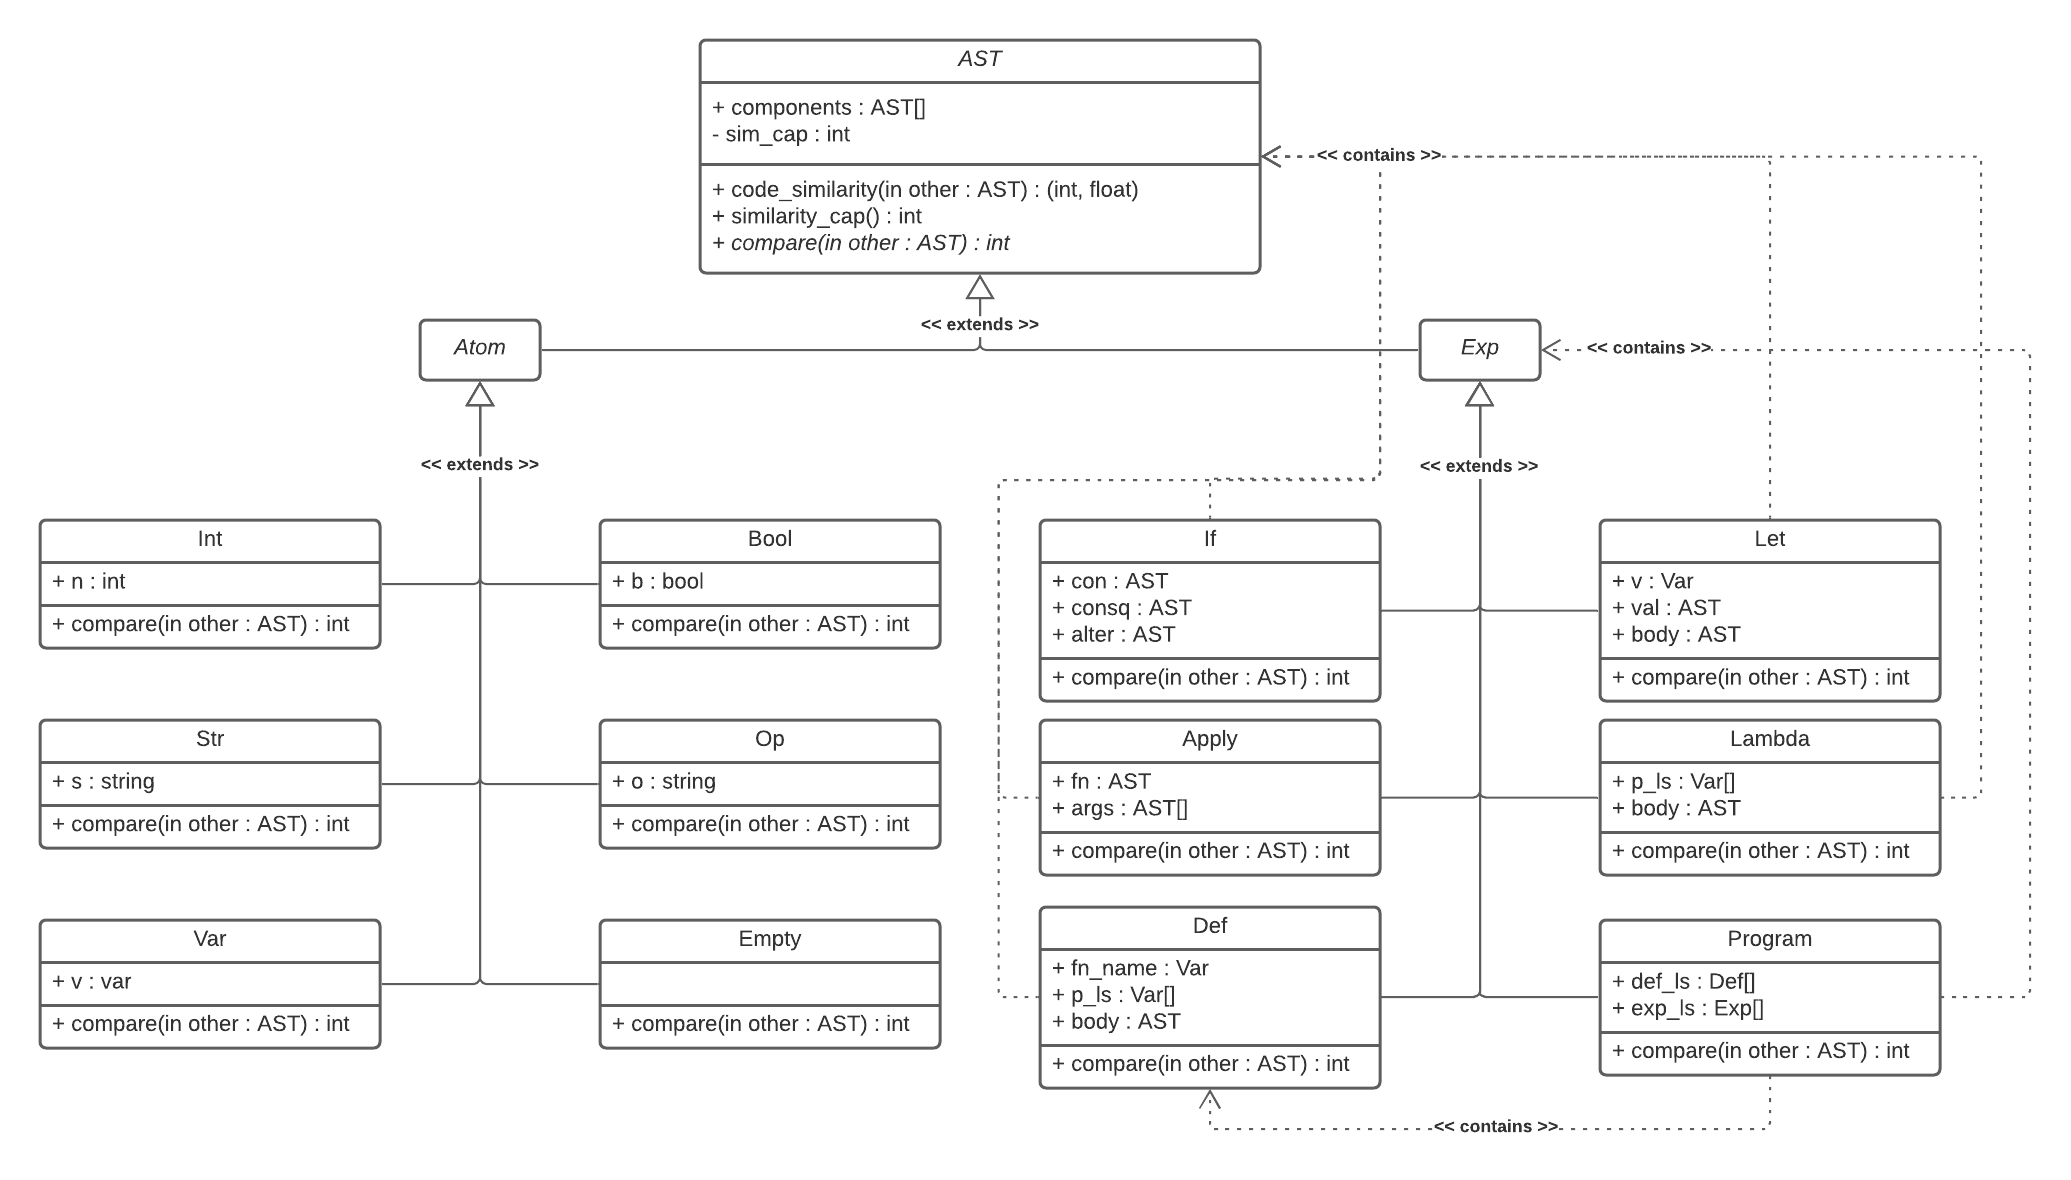
\includegraphics[scale=.45]{oop_uml}
  \end{mdframed}
  \caption{UML Diagram for OOP Design of AST}
  \label{oop-uml}
\end{figure}

In addition to the \key{struct} fields introduced in Table \ref{ast-structs}, we have added two additional fields and three new methods to \key{AST} objects. The \key{compare} method calculates the similarity score as detailed in the previous section. Likewise, \key{similarity\_cap} calculates the similarity cap. The field \key{sim\_cap} serves to allow for lazy evaluation of the similarity cap\textemdash once \key{similarity\_cap} is called once, then \key{sim\_cap} is updated with the calculated value. In all future calls to \key{similarity\_cap}, \key{sim\_cap} is returned instead of reperforming calculations. The field \key{components} is used in calculating the similarity cap; it contains all components of the node required to calculate the similarity cap so that they can be recursed on. This allows for better abstraction, as all \key{Exp} objects calculate their similarity cap in the same manner.

\hfill

While the \key{Atom} and \key{Exp} abstract classes are largely unneeded, they were included for the sake of scalability in the future. The implementations of the \key{compare} methods are fairly straightforward and follow the algorithms described in the previous section.

\subsubsection{Converting Racket AST to Python AST}

Converting Racket AST \key{structs} to Python objects is also fairly painless. We simply match on the AST nodes, create strings representing Python object construction, and recurse on the components to create the other constructors. 

\hfill

From there, we can pipe the constructed strings through \key{stdout} and into a Python script that runs Python's \key{eval} function to create the described objects.

\subsubsection{Terminal Interface and Behavior}

To interact with the similarity program, we need some sort of terminal interface that we can work with to process files for similarity. The purpose of the Code Similarity Detection Tool is to detect how similar a provided smart contract is to pre-existing popular and mature contracts. As such, it follows that we maintain a database of the aforementioned pre-existing contracts. In this project, those files would be stored in the \key{archetypes/} directory.

\hfill

The program needs to first read all of the \key{archetypes/} files and create individual ASTs for each file. Then it should ask for a single file to run the Code Similarity Detection Tool on and generate the AST from the provided file. Then simply run the comparison function between that AST and all ASTs generated from the \key{archetypes/} directory and output the pairing with the highest relative similarity.

\usection{Weaknesses and Improvements}

\subsection{Hiding Similarities in Differing Structures}
Unfortunately, this design is not without flaws. The code similarity algorithm simply returns 0 if two AST nodes are not of the same structure. This means the following example would return 0 as a code similarity score, despite being fairly similar:

\begin{figure}[H]
  \begin{mdframed}
    \begin{lstlisting}[escapechar=\%]
(let ([x 5])
  (+
    (if (< x 10)
        12
        x)
    5))

; vs

(+
  (let ([x 5])
    (if (< x 10)
        12
        x))
   5)
    \end{lstlisting}
  \end{mdframed}
  \caption{An edge-case example that shows the weakness of the algorithm.}
  \label{weak-example}
\end{figure}

It is certainly possible to ameliorate this issue\textemdash perhaps discarding the variable binding in \key{Let} structures when performing comparisons between a \key{Let} structure and a different structure could work. However, further testing would be required to determine if this causes any other issues.

\subsection{Syntactical vs Semantical Analysis}

As mentioned in the beginning of this document, this tool evaluates syntactical similarities. In other words, while it can check structural similarity, it is unable to determine if two programs behave similarly. The following two programs would score highly syntactically, despite being different semantically:

\begin{figure}[H]
  \begin{mdframed}
    \begin{lstlisting}[escapechar=\%]
(define (fib n)
  (if (<= n 1)
    1
    (+ (fib (- n 1)) (fib (- n 2)))))

; vs

(define (fact n)
  (if (<= n 1)
    1
    (* n (fact (- n 1)))))
    \end{lstlisting}
  \end{mdframed}
  \caption{Syntactical vs Semantical Analysis}
  \label{syntax-vs-sematics}
\end{figure}

Syntactical analysis, unsurprisingly, is a much simpler task than semantical analysis. Take for example, a case where two programs apply the same function, but with the arguments in different orders. Determining similarity in syntax would be simple, but determining behavioral similarity would require discerning whether the function is deterministic, commutative, etc. Furthermore, according to Rice's Theorem, fully determining behavioral equivalence of two programs is undecidable.

\subsection{Similarity Algorithm Improvements}

The similarity algorithm described previously is rather rudimentary\textemdash with a couple of tweaks and changes in weights, it could possibly be improved further. For example, when evaluating the similarity of two function applications, we could take the similarity of the applied functions and create a coefficient that is used in determining the impact of argument similarity. By doing so, we can change how the function being applied affects the similarity of the entire function application. 

\hfill

There are likely many other ways of improving on the similarity algorithm. It may even be necessary to change how the AST is constructed and how functions are treated in the De Bruijn conversion. With more experimenting, we may achieve a more accurate code similarity algorithm while preserving the core concepts outlined in this project.
\end{document}
